\documentclass[aspectratio=169]{beamer}\usepackage[]{graphicx}\usepackage[]{color}
%% maxwidth is the original width if it is less than linewidth
%% otherwise use linewidth (to make sure the graphics do not exceed the margin)
\makeatletter
\def\maxwidth{ %
  \ifdim\Gin@nat@width>\linewidth
    \linewidth
  \else
    \Gin@nat@width
  \fi
}
\makeatother

\definecolor{fgcolor}{rgb}{0.345, 0.345, 0.345}
\newcommand{\hlnum}[1]{\textcolor[rgb]{0.686,0.059,0.569}{#1}}%
\newcommand{\hlstr}[1]{\textcolor[rgb]{0.192,0.494,0.8}{#1}}%
\newcommand{\hlcom}[1]{\textcolor[rgb]{0.678,0.584,0.686}{\textit{#1}}}%
\newcommand{\hlopt}[1]{\textcolor[rgb]{0,0,0}{#1}}%
\newcommand{\hlstd}[1]{\textcolor[rgb]{0.345,0.345,0.345}{#1}}%
\newcommand{\hlkwa}[1]{\textcolor[rgb]{0.161,0.373,0.58}{\textbf{#1}}}%
\newcommand{\hlkwb}[1]{\textcolor[rgb]{0.69,0.353,0.396}{#1}}%
\newcommand{\hlkwc}[1]{\textcolor[rgb]{0.333,0.667,0.333}{#1}}%
\newcommand{\hlkwd}[1]{\textcolor[rgb]{0.737,0.353,0.396}{\textbf{#1}}}%

\usepackage{framed}
\makeatletter
\newenvironment{kframe}{%
 \def\at@end@of@kframe{}%
 \ifinner\ifhmode%
  \def\at@end@of@kframe{\end{minipage}}%
  \begin{minipage}{\columnwidth}%
 \fi\fi%
 \def\FrameCommand##1{\hskip\@totalleftmargin \hskip-\fboxsep
 \colorbox{shadecolor}{##1}\hskip-\fboxsep
     % There is no \\@totalrightmargin, so:
     \hskip-\linewidth \hskip-\@totalleftmargin \hskip\columnwidth}%
 \MakeFramed {\advance\hsize-\width
   \@totalleftmargin\z@ \linewidth\hsize
   \@setminipage}}%
 {\par\unskip\endMakeFramed%
 \at@end@of@kframe}
\makeatother

\definecolor{shadecolor}{rgb}{.97, .97, .97}
\definecolor{messagecolor}{rgb}{0, 0, 0}
\definecolor{warningcolor}{rgb}{1, 0, 1}
\definecolor{errorcolor}{rgb}{1, 0, 0}
\newenvironment{knitrout}{}{} % an empty environment to be redefined in TeX

\usepackage{alltt}
\usetheme{berlin}
\usepackage{graphicx}
\title[Bayesian Mixed Models]{Efficient Bayesian mixed-model analysis increases association power in large cohorts}
\author[Dominic LaRoche]{Loh et al. 2015.  Nature Genetics}
\IfFileExists{upquote.sty}{\usepackage{upquote}}{}
\begin{document}

\maketitle

\section{Introduction}
\begin{frame}{Mixed-models in GWAS}
\begin{itemize}
\item Linear mixed models (LMM) have become increasingly popular for genome-wide association studies (GWAS)
\pause
\item Variance components can account for inherently hierarchical data
\pause
\begin{itemize}
\item Observations are, by definition, not independent
\item Dependence structure is not always known \emph{a priori}
\begin{itemize}
\item \small{(sometimes cousins unwittingly wed)}
\item Dependence structure can be estimated from the data
\end{itemize}
\end{itemize}
\pause
\item LMMs can reduce the false discovery rate by accounting for pseudo-replication
\pause
\item LMMs can be computationally expensive, $O(MN^2)$ or $O(M^2N)$
\end{itemize}
\end{frame}

\begin{frame}{Standard LMM}
The standard LMM takes the form:
$$y_i = x_{i}\beta + \sigma^2_GK + \sigma^2_EI$$
Where $y_i$ is the phenotype of individual $i$, $x{i}$ are the covariates of interest (SNPs, age, etc.), $\sigma^2_G$ is the variance due to genetic similarity, $K$ is the \emph{genetic similarity matrix (GSM)}, $E$ is the variance due to environment (chance), and $I$ is the NxN identity matrix.

\begin{itemize}
\item The GSM ($K$) accounts for the hierarchical structure of the data and can be estimated in various ways
\item The $ \sigma^2_EI$ term is similar to a typical regression error term
\end{itemize}
\end{frame}

\begin{frame}{LMM Model Assumptions}
\begin{itemize}
\item Assumes the "infinitesimal model" of genetic effects
\pause
\begin{itemize}
\item Proposed by Fisher in 1930
\item Many loci contribute small additive effects for a phenotype
\item Appears consistent with some traits (size) but not others (Huntington's disease)
\end{itemize}
\pause
\item Assumes correctly specified variance components
$$\sigma^2_G \text{ and } \sigma^2_E$$
\pause
\item Assumes linearity in the parameters ($\beta$)
\end{itemize}
\end{frame}

\begin{frame}{LMM Test Statistic}
For efficiency the current methodology incorporates a 2 step process:
\pause
\begin{itemize}
\item[1] Fit the variance components via REML ($\sigma^2_GK$ and $\sigma^2_EI$).
\pause
\item[2] Use score test to compute test statistics for each SNP
$$\chi^2_1 = \frac{\left(x^{\prime}_{SNP}V^{-1}y\right)^2}{x^{\prime}_{SNP}V^{-1}x_{SNP}}$$

where $V$ is the $cov(y) =  \sigma^2_GK + \sigma^2_EI$
\end{itemize}
(Some models use simultaneous likelihood ratio tests to achieve exact statistics)
\end{frame}

\section{Methods}

\begin{frame}{Proposed Model}
Proposed model has the same basic components:
$$y_i = x_{i}\beta + \sigma^2_GK + \sigma^2_EI$$
\pause
\begin{itemize}
\item Several ``improvements":
\begin{itemize}
\item[1] Adjust current score statistic with calibration factor, $c$.
\item[2] Test against ``denoised" residuals for increased power
\item[3] Gaussian mixture extension to accommodate heterogeneous effect sizes
\end{itemize}
\pause
\item Not purely Bayesian -- actual test statistic is frequentist
\end{itemize} 
\end{frame}

\begin{frame}{Calibration Factor: $c_{inf}$}
The BOLT\_LMM statistic (for infinitesimal model)
$$\chi^2_1 = \frac{\left( x^{\prime}_{SNP}V^{-1}_{LOCO}y\right)^2}{c_{inf}}$$
where, 
$$c_{inf} = \frac{\text{mean}\left(x^{\prime}_{SNP}V^{-1}_{LOCO}y\right)^2}{\text{mean}\chi^2_1}$$

This statistic is similar to others (GRAMMAR-gamma and MASTOR) but avoids proximal contamination via the LOCO approach.
\end{frame}

\begin{frame}{Key Insight}
The key insight in this paper is this approach:
\smallskip
\begin{itemize}
\item The numerator from the $\chi^2$ statistic is a scalar multiple of $\sigma^2_EV^{-1}_{LOCO}y$
\smallskip
\pause
\begin{itemize}
\item The test statistic uses residuals where other effects have been ``conditioned out"
\pause
\item Less noise = more power to detect a signal
\pause
\item Can manipulate the model producing the residual without changing the test statistic
\pause
\end{itemize}
\smallskip
\item The test statistic is still a quasi-likelihood score so is asymptotically $\chi^2$ 
\end{itemize}
\end{frame}

\begin{frame}{The Bayesian Part}
Assume the effects, $\beta$ have a distribution:
\begin{itemize}
\item Infinitesimal model:
$$\beta \sim N(0,\sigma^2_{G})/M$$
where $M$ is the proximally-controlled SNPs under evaluation
\pause
\smallskip
\item The general (heterogeneous effects) model utilizes a Gaussian mixture:
$$\beta \sim N(0,\sigma^2_{\beta,1}) \text{ with probability }p$$
$$\beta \sim N(0,\sigma^2_{\beta,2}) \text{ with probability }1-p$$

If p is small and $\sigma^2_{\beta,2}$ is much smaller than $\sigma^2_{\beta,1}$ you will get a many $\beta$s of small (near 0) effect and a few of large effect.
\end{itemize}
\end{frame}

\begin{frame}{From Bayesian to Frequentist}
The method uses Bayesian model to obtain a frequentist statistic:
\begin{itemize}
\item First fit the Bayesian mixture model
\item Calculate the posterior mean to obtain the residual
\item Use the residual to calculate the $\chi^2$ statistic
\end{itemize}
\end{frame}

\section{Results}

\begin{frame}{Computational Efficiency}
\begin{columns}[onlytextwidth]
\begin{column}{0.6\textwidth}
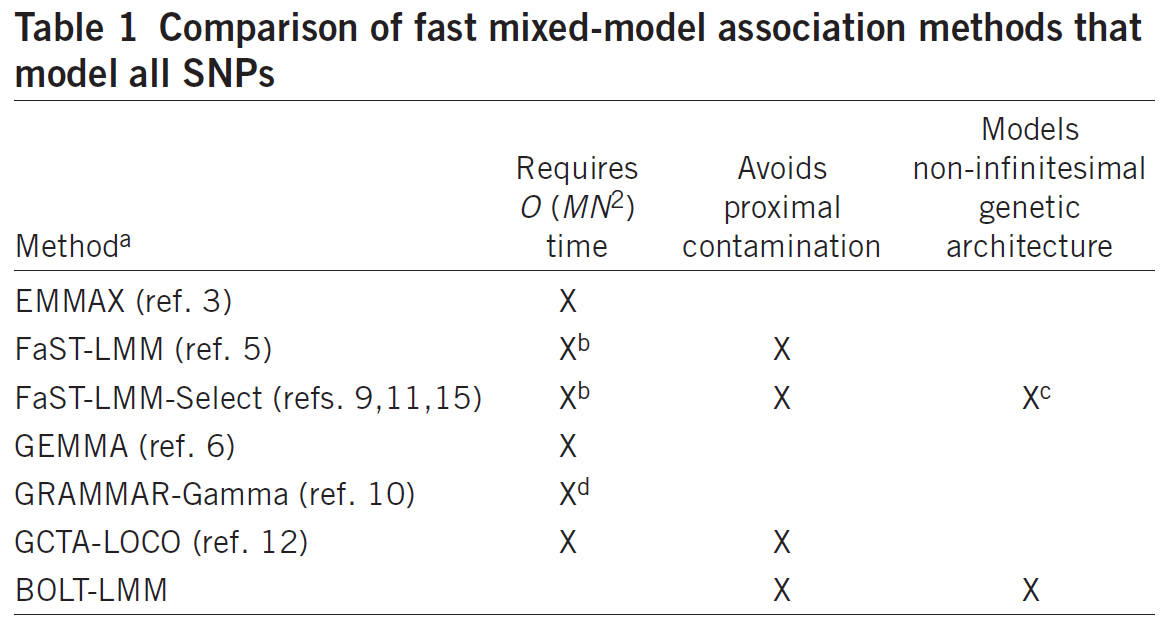
\includegraphics[scale=.25]{./figure/Table1.png}
\end{column}
\begin{column}{0.4\textwidth}
\begin{itemize}
\item Computes on $\sim O(MN)$ time
\item Avoids proximal contamination by borrowing methods from GCTA-LOCO
\item Accommodates non-infinitesimal genetic architecture
\end{itemize}
\end{column}
\end{columns}
\end{frame}

\begin{frame}{Computational Efficiency}
\begin{columns}[onlytextwidth]
\begin{column}{0.5\textwidth}
\begin{itemize}
\item Fastest of the group*
\item CPU time scales to $\sim O(MN^{1.5})$
\item Memory use scales to $\sim O(MN)$
\end{itemize}
\end{column}
\begin{column}{0.5\textwidth}
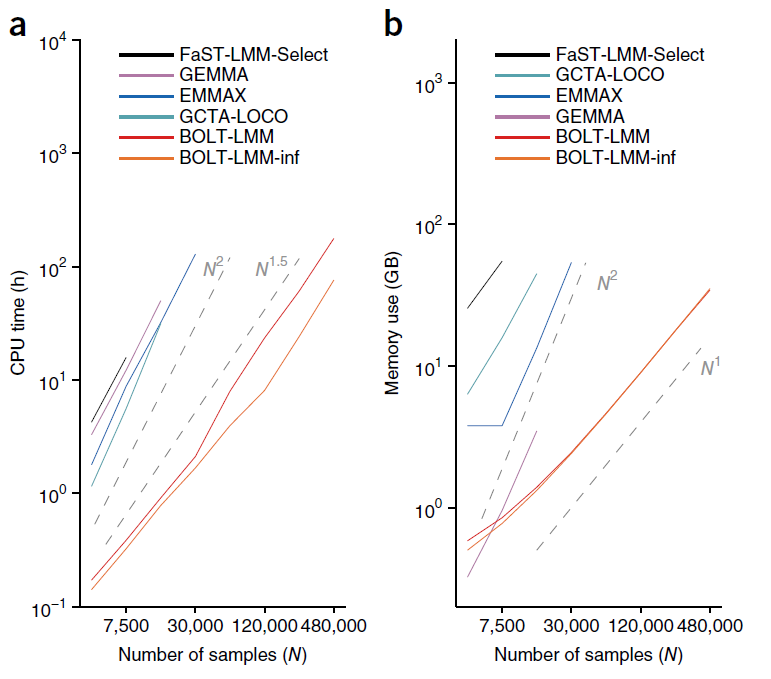
\includegraphics[scale=.3]{./figure/CompTimeFig.png}
\end{column}
\end{columns}
\end{frame}


\begin{frame}{Simulations}
\begin{columns}[onlytextwidth]
\begin{column}{0.6\textwidth}
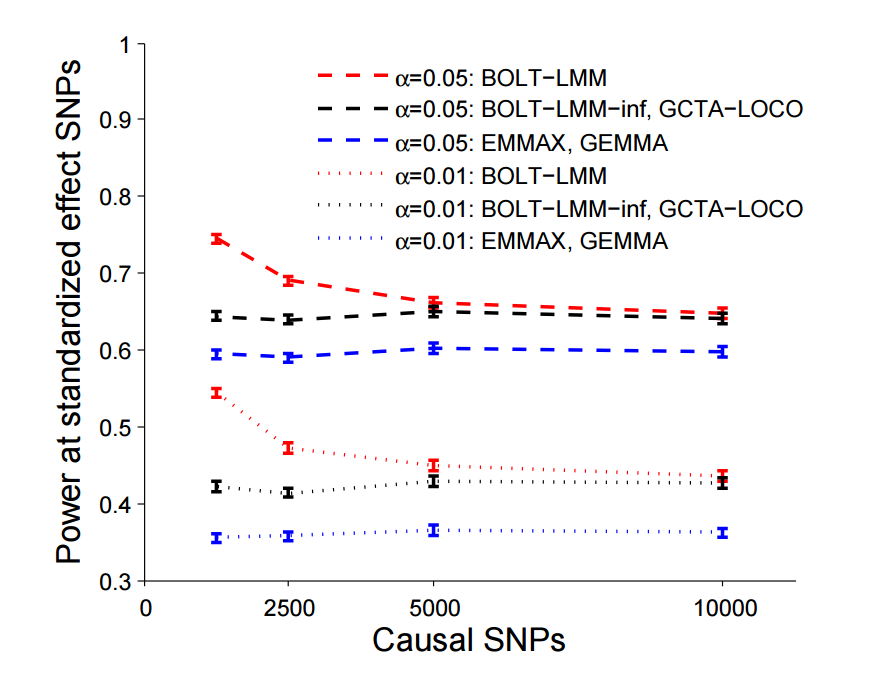
\includegraphics[scale=.3]{./figure/PowerCurves.png}
\end{column}
\begin{column}{0.4\textwidth}
\begin{itemize}
\item Increased power especially when the number of causal SNPs is small
\item Increased power is stable at various $\alpha$ levels (consistent with theory)
\item BOLT-LMM is virtually identical to GCTA-LOCO under infinitesimal architecture assumption
\end{itemize}
\end{column}
\end{columns}
\end{frame}

\begin{frame}{Simulations}
\begin{columns}[onlytextwidth]
\begin{column}{0.5\textwidth}
\begin{itemize}
\item Effective false positive control
\item Large gains in power with small number of causal SNPs
\item No associated increase in type I error with power increase
\end{itemize}
\end{column}
\begin{column}{0.5\textwidth}
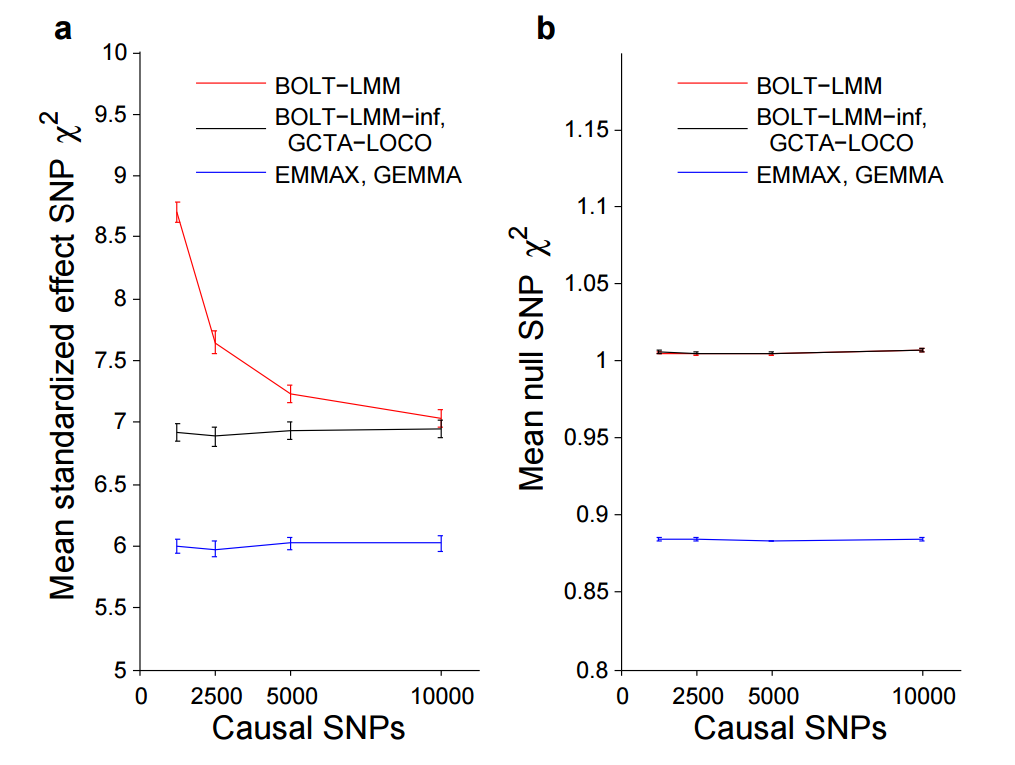
\includegraphics[scale=.25]{./figure/FalsePositiveControl.png}
\end{column}
\end{columns}
\end{frame}

\begin{frame}{Women's Genome Health Study}
\begin{columns}[onlytextwidth]
\begin{column}{0.5\textwidth}
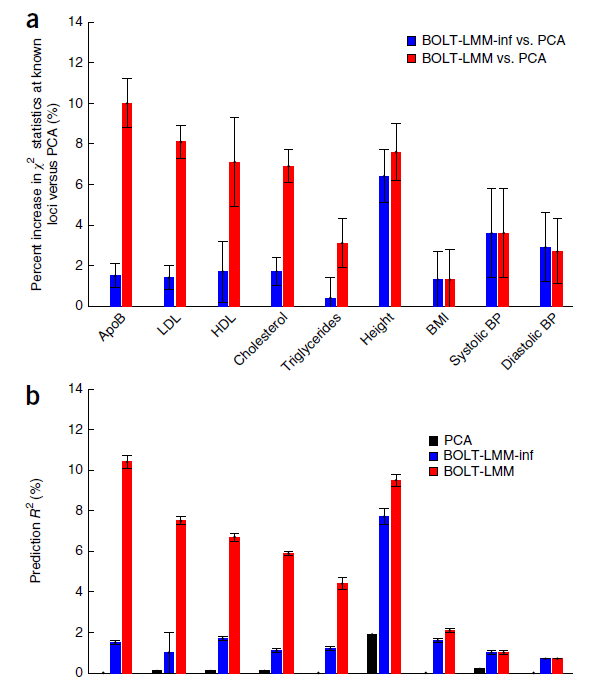
\includegraphics[scale=.3]{./figure/WGHSPerf.png}
\end{column}
\begin{column}{0.5\textwidth}
\begin{itemize}
\item Similar increases in power in non-simulated data
\item Power increases are not homogeneous (as predicted by theory) 
\item Substantial increases in predictive ability
\end{itemize}
\end{column}
\end{columns}
\end{frame}

\section{Discussion}

\begin{frame}{Comments from the Peanut Gallery}
\begin{itemize}
\item Not sure about mixing Bayesian and Frequentist paradigms
\bigskip
\item Room to improve the modelling of genetic architecture
\bigskip
\item Carry the Bayesian theme through to the test statistic to get a credible interval
\end{itemize}
\end{frame}

\begin{frame}
\begin{columns}[onlytextwidth]
\begin{column}{0.5\textwidth}
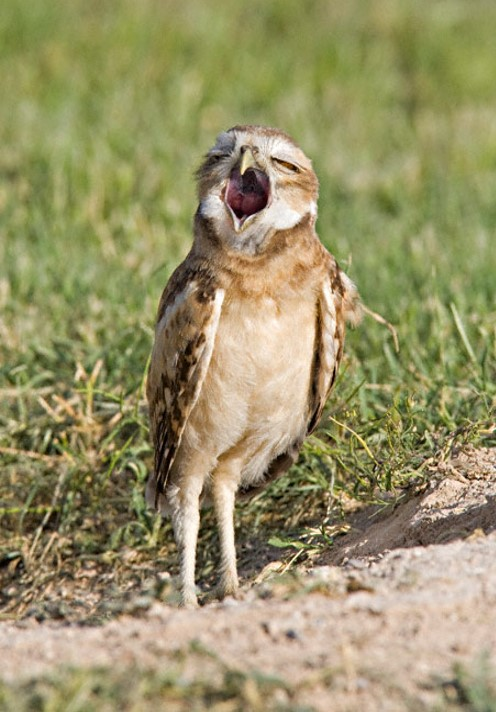
\includegraphics[scale=.6]{./figure/YawningOwl.jpg}
\end{column}
\begin{column}{0.5\textwidth}
\huge Questions?
\end{column}
\end{columns}
\end{frame}

\end{document}
